%%% TeX-master: "manuscript"
% !TeX spellcheck=en_GB

\newpage

\section*{Figures}

\subsection*{Figure 1}

\begin{figure}[ht]
  \centering
  \includegraphics{fig_1_pathway_overview}
  
  \label{fig:pathway_overview}
\end{figure}

\newpage


\subsection*{Figure 2}

\begin{figure}[ht]
  \centering
  \includegraphics[width=0.75\textwidth]{fig_2_phylo_distribution}
 
  \label{fig:phylo_distribution}
\end{figure}

\newpage


\subsection*{Figure 3}

\begin{figure}[ht]
  \centering
  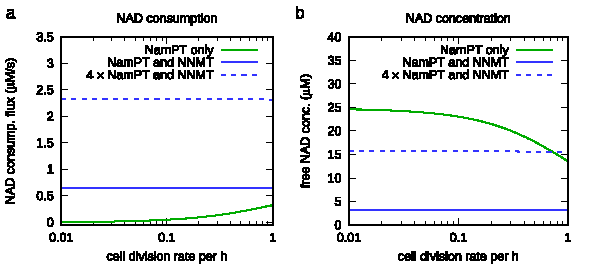
\includegraphics[width=\textwidth]{fig_3_NNMT_NAD_flux}
 
  \label{fig:NNMT_NAD_flux}
\end{figure}

\newpage


\subsection*{Figure 4}

\begin{figure}[ht]
  \centering
  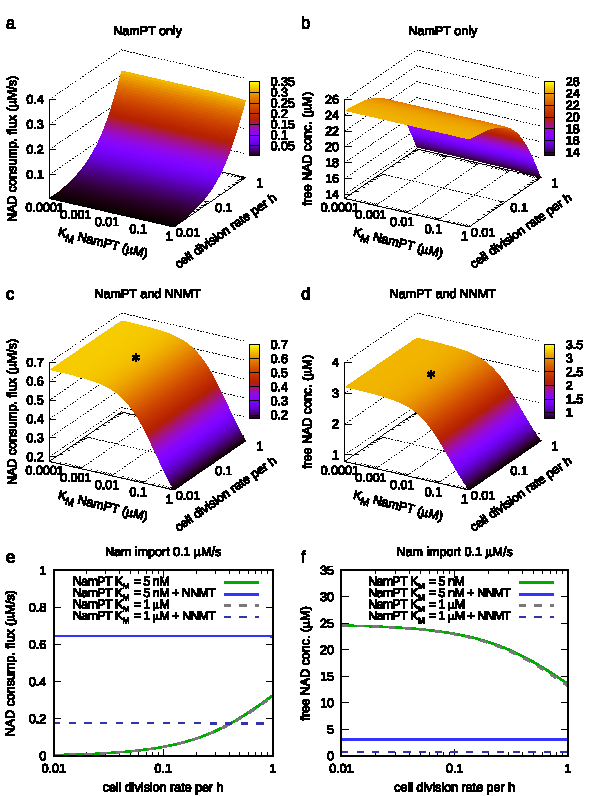
\includegraphics[width=0.72\textwidth]{fig_4_NamPRT_affinity_Nam}

  \label{fig:NamPT_affinity_Nam}
\end{figure}

\newpage


\subsection*{Figure 5}

\begin{figure}[ht]
  \centering
  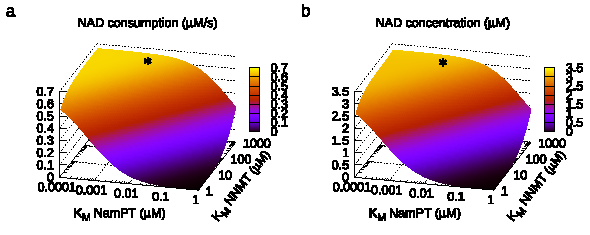
\includegraphics[width=\textwidth]{fig_5_optimal_substr_affinities}
 
  \label{fig:optimal_substr_affinities}
\end{figure}

\newpage


\subsection*{Figure 6}

\begin{figure}[ht]
  \centering
  \includegraphics[width=0.83\textwidth]{fig_6_unresolved_loop}
\end{figure}

\newpage

\begin{figure}[ht]
 
  \label{fig:unresolved_loop}
\end{figure}



\subsection*{Figure 7}

\begin{figure}[ht]
  \centering
  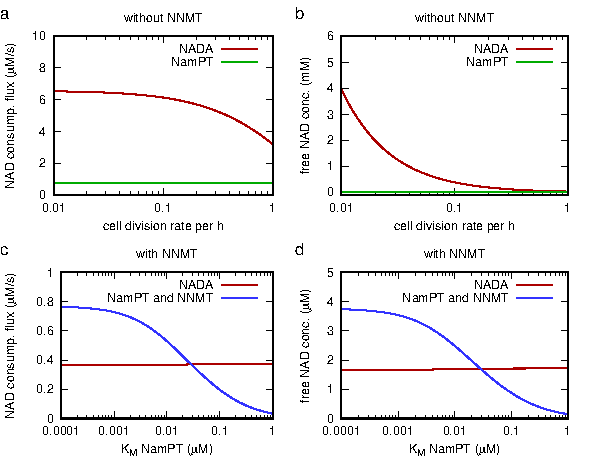
\includegraphics[width=\textwidth]{fig_7_NNMT_comp_advantage}
 
  \label{fig:NNMT_comp_advantage}
\end{figure}

\newpage


\subsection*{Figure 8}

\begin{figure}[ht]
  \centering
  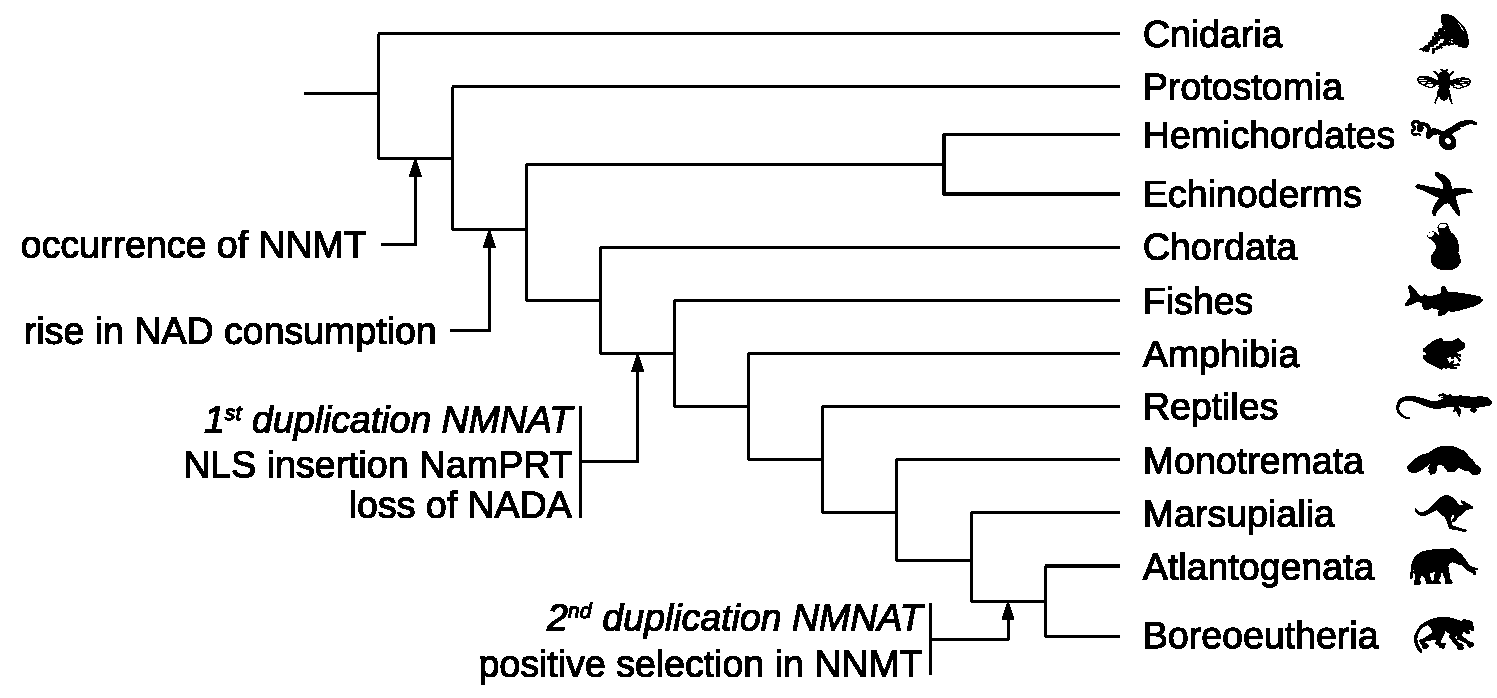
\includegraphics[width=\textwidth]{fig_8_evo_events}
 
  \label{fig:evo_events}
\end{figure}
